\chapter{Implementation} \label{chap:impl}

\section{Duties and Agreements}

To successfully write your thesis, you should definitely respect some rules. They are explained in the following sections.

\subsection{Rules for Students}
At the beginning of your thesis, estimate the complexity of the work you are going to have. Take into account that you will have problems with certain aspects of your thesis that will consume a lot of time. Consider times for recreation and delays you can not influence, for instance, asking your supervisor, waiting for orders to be shipped, complex problems during the implementatuon phase, and so on~\dots

For some students it is a good idea to agree upon a rough plan (with their supervisor) on how to make progress on their thesis and what goals to achieve. Milestones might help to control your progress. If you fail to meet a milestone in time, contact your supervisor on why this happened or when to expect it to be fulfilled.

If you have a problem, try to solve it on your own twice over. Some things just take time. In case you fail to solve it on your own, write an email to your supervisor and tell him about your problem and what you did to solve it. Make an appointment if necessary. Please do not jump right into his office, supervisors have other stuff to do, too.

For quotations, either use ``quotation'' or \enquote{quotation}. For some words, you should use a tilde to link them, for example, when referring to chapter~\ref{chap:conclusion} you should use it. Or use \autoref{chap:conclusion}. This prevents words from being separated by a line break or some other rare circumstances. Use BibTeX within your thesis and learn the different citation options~\cite{Xie:2008:SBS,Newsome:05:DTA}. 

One last piece of advice. Do not try to attend courses in parallel to your thesis. You should take this seriously and not think that writing a thesis is done quickly.

\subsection{Rules for Supervisors}
\enquote{With great power comes great responsibility} \texttt{:-)}

\begin{itemize}
\item It is very important, that if you want specific things to be done that you send these important instructions by mail. Your student might be in a moment of confusion when telling him.
\item Attend the \enquote{Diplomandenseminar} and give your student the feeling, that this is important to you, too.
\item Offer your students the opportunity to talk to you right after the \enquote{Diplomandenseminar}. While discussing things, tell your student to write down the results of this discussion and tell him to send you this summary by mail to ensure (if necessary), you did not talk at cross purposes.
\item Last but not least: Please be gentle to your students \texttt{:-)}
\end{itemize}

\section{Hints on Typesetting}
To get this template running, you need at least

\begin{itemize}
\item either TeXLive 2010 (use update utility and install the most recent packages!)
\item or MikTeX (\textcolor{red}{IMPORTANT}: install the cm-super font package manually!)
\end{itemize}

This template is confirmed to work in both situations. In case it does not work for you, there is something wrong with your \LaTeX\/ environment \texttt{:-)}\\

You can use \texttt{pdflatex} or \texttt{latex} to typeset this template.

\subsection{Structuring Text, English Hints}
Another text about the following sections \dots

\subsubsection{Text }
Always try to structure your text in a manner that makes sense. Either use indentations, itemize or enumeration environments.

This sentence will have an indentation at the beginning. Now an enumeration starts:

\begin{enumerate}
\item One.
\item Two.
\item Three.
\end{enumerate}

\noindent Sometimes you do not want an indentation. Use the \texttt{noindent} command in such a case.

\paragraph{One} Is the first number. 

\paragraph{Two} Is the second number.

\subsubsection{English Hints}

\begin{itemize}
\item Use an active voice and avoid using passive wherever possible.
\item \emph{Always} use the present tense (especially when you refer to content that occurs later in your text). For example:
	\begin{itemize}
	\item \emph{wrong}: The next chapter \emph{will} explain \dots
	\item \emph{correct}: The next chapter explains \dots
	\end{itemize}
\item Either use American English or British English, but do not mix (e.\,g. summarize vs. summarise, analyze vs. analyse, \dots). American English is preferred.
\item Do not use filler words.
	\begin{itemize}
	\item omit: \enquote{some kind of} and others \dots
	\end{itemize}
\item Never use a comma before \enquote{that}.
\item For enumerations, always use a comma before \enquote{and}: \enquote{\dots module 1, module 2, and module 3.}.
\item The title of your thesis is capitalized except for words like and, or, with, the, a \dots
\item \emph{Always} address the reader using the third person: \enquote{As one can see from \dots} and not \enquote{As you can see \dots}.
\item All tables, figures have to be explained very briefly in the text itself.
\item Always use correct quantifications:
	\begin{itemize}
	\item \emph{wrong}: \dots a small amount of runs \dots
	\item \emph{correct}: \dots at most three runs \dots
	\end{itemize}
\item Never use \enquote{I}. Depersonalize your sentences or use \enquote{we} if necessary.
\item Read \emph{The Elements of Style} by William Strunk, Jr., which is for example available at \url{http://www.crockford.com/wrrrld/style.html}. The (short) book provides an overview of typical errors and helps you to significantly improve your English.
\end{itemize}

\subsubsection{General Hints}
\begin{itemize}
 \item Use non-breaking small space for some abbreviation
 \begin{itemize}
 \item z.\,B.
 \item u.\,a.
 \item e.\,g.
 \end{itemize}
 \item Use a non-breaking space just before references, parentheses and so which shall not begin at the beginning of a new line. This sentence will not break~here~(and~here).
 \item Did you notice the overfull horizontal box (hbox)? You should avoid these! Underfull boxes are not that bad. But only fix them when most of the section, paragraph etc is ready. Otherwise you have to fix them more than once. You can tell \LaTeX\ when to break a word if it does not do it correctly. Just put a \textbackslash- at the corresponding position in the world. Vertical overfull boxes (vbox) occur if the document uses \verb|\flushbottom| instead of \verb|\raggedbottom|. That way, \LaTeX\ ensures that each page ends with the last sentence in the last line (except for the final line in a section). To enforce this, \LaTeX\ sometimes has to add extra vertical space between, e.\,g., paragraphs. Overfull vertical boxes are hard to fix, as additional content needs to be added or even has to be removed sometimes. Keep in mind that any changes to the type area (Satzspiegel) might produce many additional over- or underfull boxes (and of course it will fix other boxes).
 \item Read \url{ftp://ftp.dante.de/tex-archive/info/german/l2tabu/l2tabu.pdf}. Really, read it.
 \item You can find many more good information at \url{http://www.dante.de/CTAN/info/lshort/german/l2kurz.pdf}
 \item The KomaScript guide is very useful: \url{ftp://ftp.dante.de/pub/tex/macros/latex/contrib/koma-script/scrguide.pdf}
\end{itemize}


\subsection{Formulas, Figures, Tables, Definitions}

\subsubsection{Formulas}

Define abbrevations with the \verb+\acro{...}+ command, use them in the text mostly with \verb+\ac{...}+. (Yes, in this example there are still a lot of wrong abbrevations. Make it better :)

So, testing abbrevations \gls{json} is written in different form. Lets see, when using \gls{json} again, what will happen :D .

Using the method shown in Table~XX for all three functions yields.
\begin{align}
f_a^4 &= \mathrm{\texttt{0x2C79}} = \mathrm{abc} + \mathrm{ac} + \mathrm{ad} + \mathrm{bc} + \mathrm{a} + \mathrm{b} + \mathrm{d} + \mathrm{1} \\
f_b^4 &= \mathrm{\texttt{0x6671}} = \mathrm{abd} + \mathrm{acd} + \mathrm{bcd} + \mathrm{ab} + \mathrm{ac} + \mathrm{bc} + \mathrm{a} + \mathrm{b} + \mathrm{d} + \mathrm{1}\\
\begin{split}
f_c^5 &= \mathrm{\texttt{0x7907287B}} = \mathrm{cde} + \mathrm{abde} + \mathrm{ade} + \mathrm{de} + \mathrm{abce} + \mathrm{bce} + \mathrm{ce} + \mathrm{be} + \mathrm{bcd}\\
&\hspace{2.75cm}+ \mathrm{acd} +\mathrm{bd} + \mathrm{d} + \mathrm{bc} + \mathrm{ab} + \mathrm{b} + \mathrm{1}
\end{split}
\end{align}

When typesetting formulas, pay special notice on constants, variables, and units:

 \begin{align}
  \mathcal{F}_{\omega}\{x(t)\} = \int^{\infty}_{-\infty} x(t) \;\mathrm{e}^{-\mathrm{j} \omega t}\,\mathrm{d}t
  \tag{Fourier-Transformation} %optional
  \end{align}
  
The use of constants, variables and units is explained by \enquote{Rohde \& Schwarz} in their famous document \enquote{Der korrekte Umgang mit Gr\"{o}\ss{}en, Einheiten und Gleichungen}~\cite{steuck2002xxe}. These rules are in compliance with ISO-31. Consequently, always typeset the following in italics:

\begin{itemize}
\item Variables like $k$, $x$, \dots
\item Functions like $f(x)$,\dots
\item Physical constants like $c_0$, \dots
\item Indices that are variables or physical units, like $a_{i, j}$ or $c_V$.
\end{itemize}

Always typeset the following upright:

\begin{itemize}
\item Functions with fixed name like $\sin(x)$ or $\Gamma (x)$.
\item Mathematical constants like $\uppi$, $\mathrm{i}$ or $\mathrm{e}$.
\item Units and their prefixes, like $\lambda = 0.56\,\upmu\mathrm{m}$, alternatively $\lambda = \SI{0.56}{\micro m}$.
\item Indices that represent names or identifiers, like $x_\mathrm{max}$ or $\mu_\mathrm B$.
\end{itemize}
  
In case it is necessary to make heavy use of user defined functions, one should use \texttt{\textbackslash\/DeclareMathOperator} to define the corresponding function. Finally, a good example how it should \emph{not} look like.

\[
Throughput = 30 mbit/s
\]

In case you need some extra symbols: \url{http://mirror.ctan.org/info/symbols/comprehensive/symbols-a4.pdf}

\subsubsection{Figures}

Figures and tables are important to explain things. Here are some rules that apply, when using figures:

\begin{itemize}
\item Whenever possible use vector graphics (eps, pdf, svg, \ldots) instead of bitmap graphics (jpg, gif, \ldots).
\item All figures should have the same font and size (do not scale them or the size will change) and ``style'' (line strength, arrow heads, \ldots).
\item Some employees of the chair need all figures in \texttt{.eps}. However, do \emph{not} convert your \texttt{.jpg} and \texttt{.png} to \texttt{.eps}, instead use a \emph{wrapper} program to wrap these file types into the \texttt{.eps} format. As a consequence, you are forced to use \texttt{latex} to typeset your document instead of \texttt{pdflatex}. Appropriate wrapper programs can be found here:
\begin{itemize}
\item Windows: \href{https://wiki.crypto.rub.de/WikiCosy/img_auth.php/6/60/JPG-PNGtoEPS.rar}{click}
\item Linux/Mac: \href{http://imgtops.sourceforge.net/}{click}
\end{itemize}
\item \textbf{Always} try to use your own figures, so you do not run into copyright problems and it is easier for us, to reuse these figures for papers. You might want to have a look at these tools to create your own figures:
	\begin{itemize}
	\item Windows: MS Visio (available via MSDNAA), Graphviz, Gnuplot \dots
	\item Linux: xfig/jfig, IPE, Graphviz, Gnuplot \dots
	\item Mac: IPE, Graphviz, Gnuplot, OmniGraffle (commercial, academic licensing available) \dots
	\end{itemize}
\end{itemize}

There are many possibilities on how to include figures, here is just one example on how to do it. In case you need further assistance, please google for \texttt{l2picfaq}.


% THIS IS A COOL AND DIRTY HACK FOR PDFLATEX USERS :-)
% LATEX USERS ARE NOT ABLE TO USE THIS
% TYPESET THIS DOCUMENT USING BOTH METHODS AND SEE THE DIFFERENCE

\ifpdf
\newpage

\KOMAoptions{pagesize,paper=landscape,DIV=20} 
\thispagestyle{empty}
\vspace*{2cm}
\begin{figure}[htbp]
	\centering
		%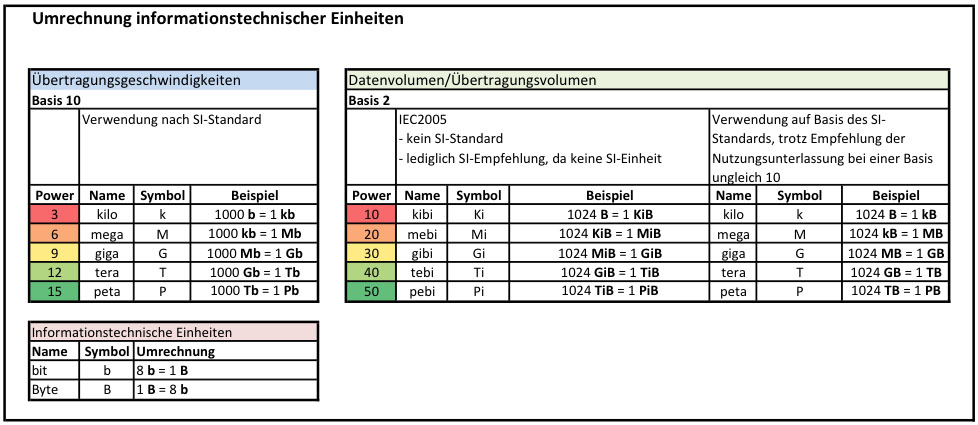
\includegraphics[scale=0.75]{images/Informationstechnische_Einheiten}
	\caption{Captions for figures are \emph{always below} the figure and give a short but informative description of the figure. Always use full sentences here and end them with a full stop. This figure explains the usage of bits and bytes in different use cases.}	
	\label{fig:emseclogo}
\end{figure}

\newpage
\KOMAoptions{paper=a4,paper=portrait,DIV=10}

\else

\begin{figure}[htbp]
	\centering
		%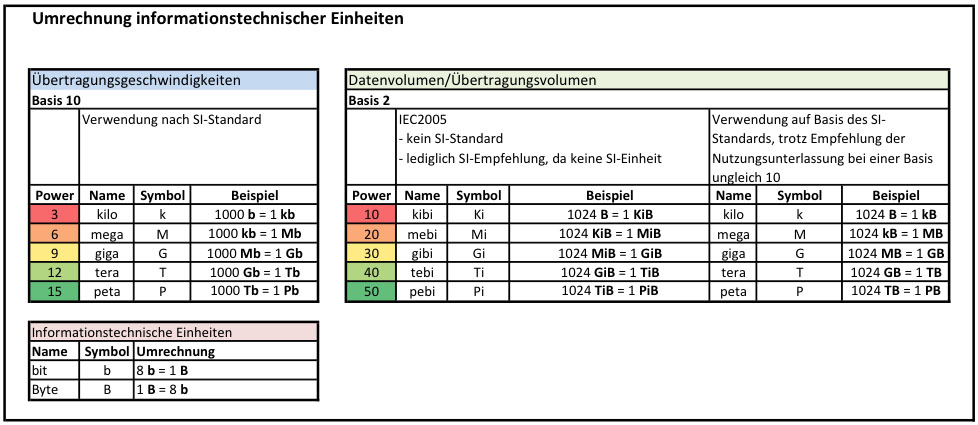
\includegraphics[scale=1.35,angle=90]{images/Informationstechnische_Einheiten}
	\caption{Captions for figures are \emph{always below} the figure and give a short but informative description of the figure. Always use full sentences here and end them with a full stop. This figure explains the usage of bits and bytes in different use cases.}	
	\label{fig:emseclogo}
\end{figure}

\fi

\begin{figure}[p]
  \centering
  \hfill %
  \subfloat[Opened Nissan car key.]{
      %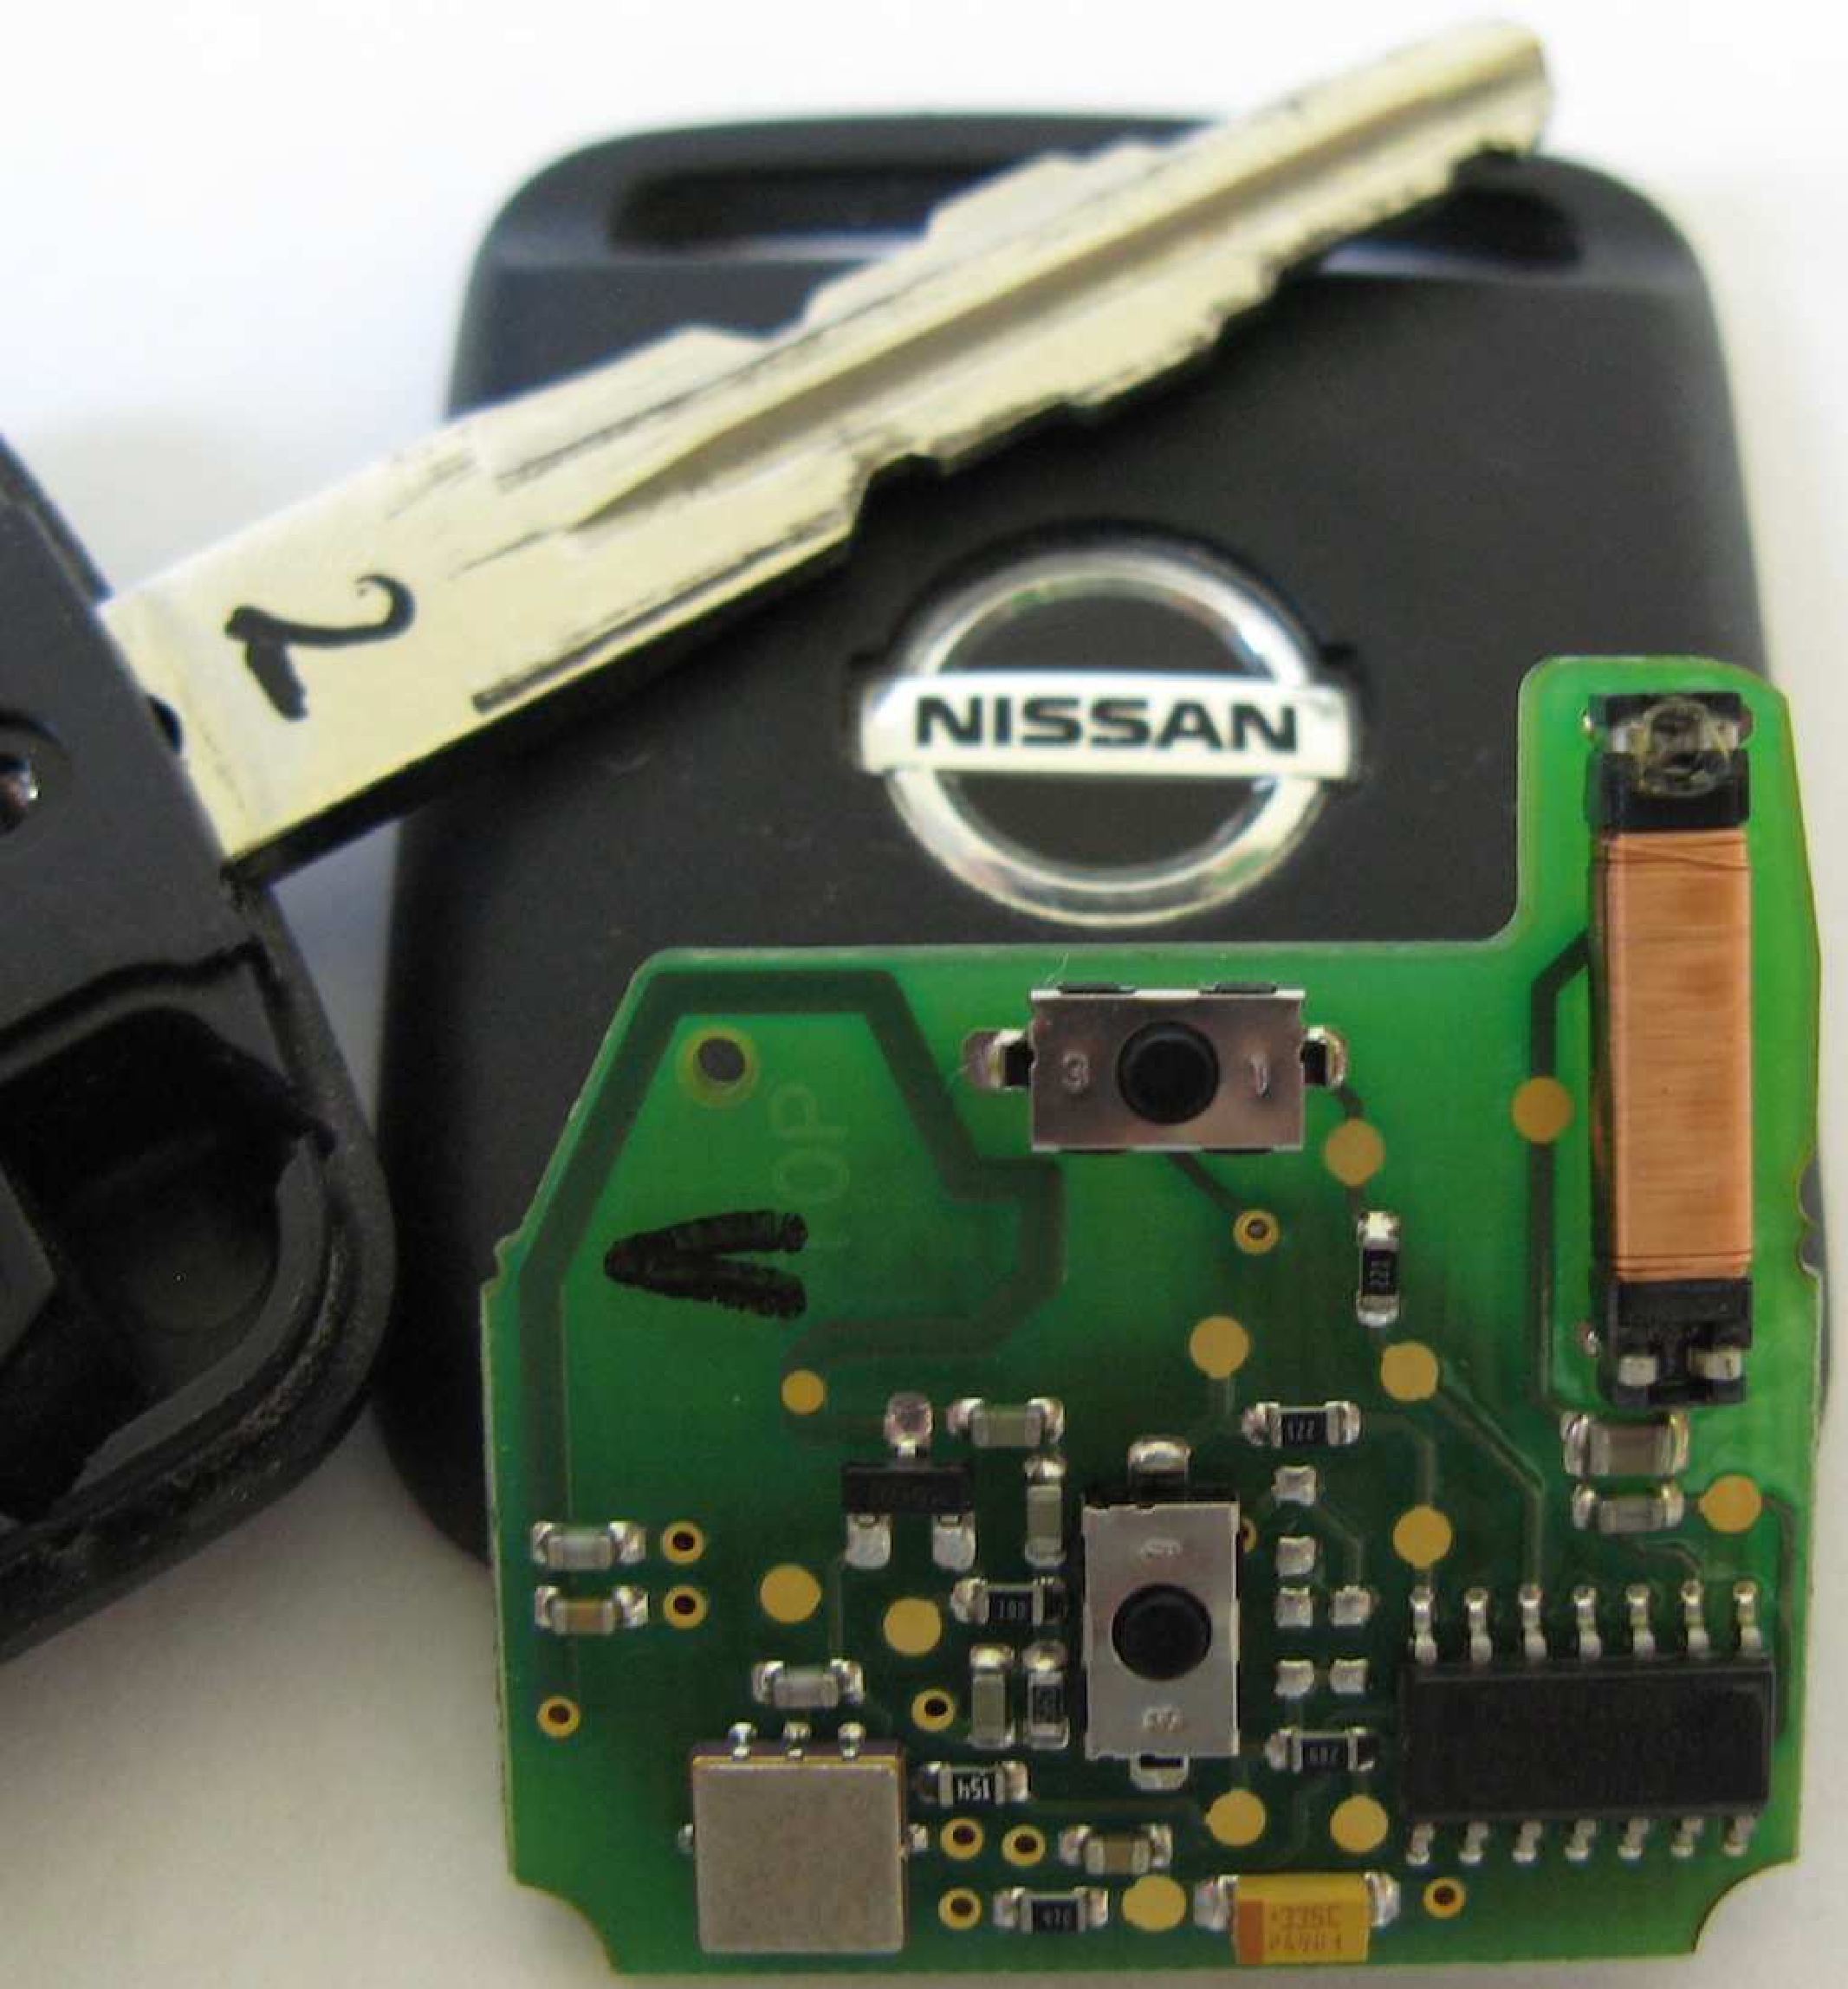
\includegraphics[width=2.35in]{images/NissanSchluessel1}
  }
  \hfill %
  \subfloat[Closeup of the transponder (PCF7946).]{
      %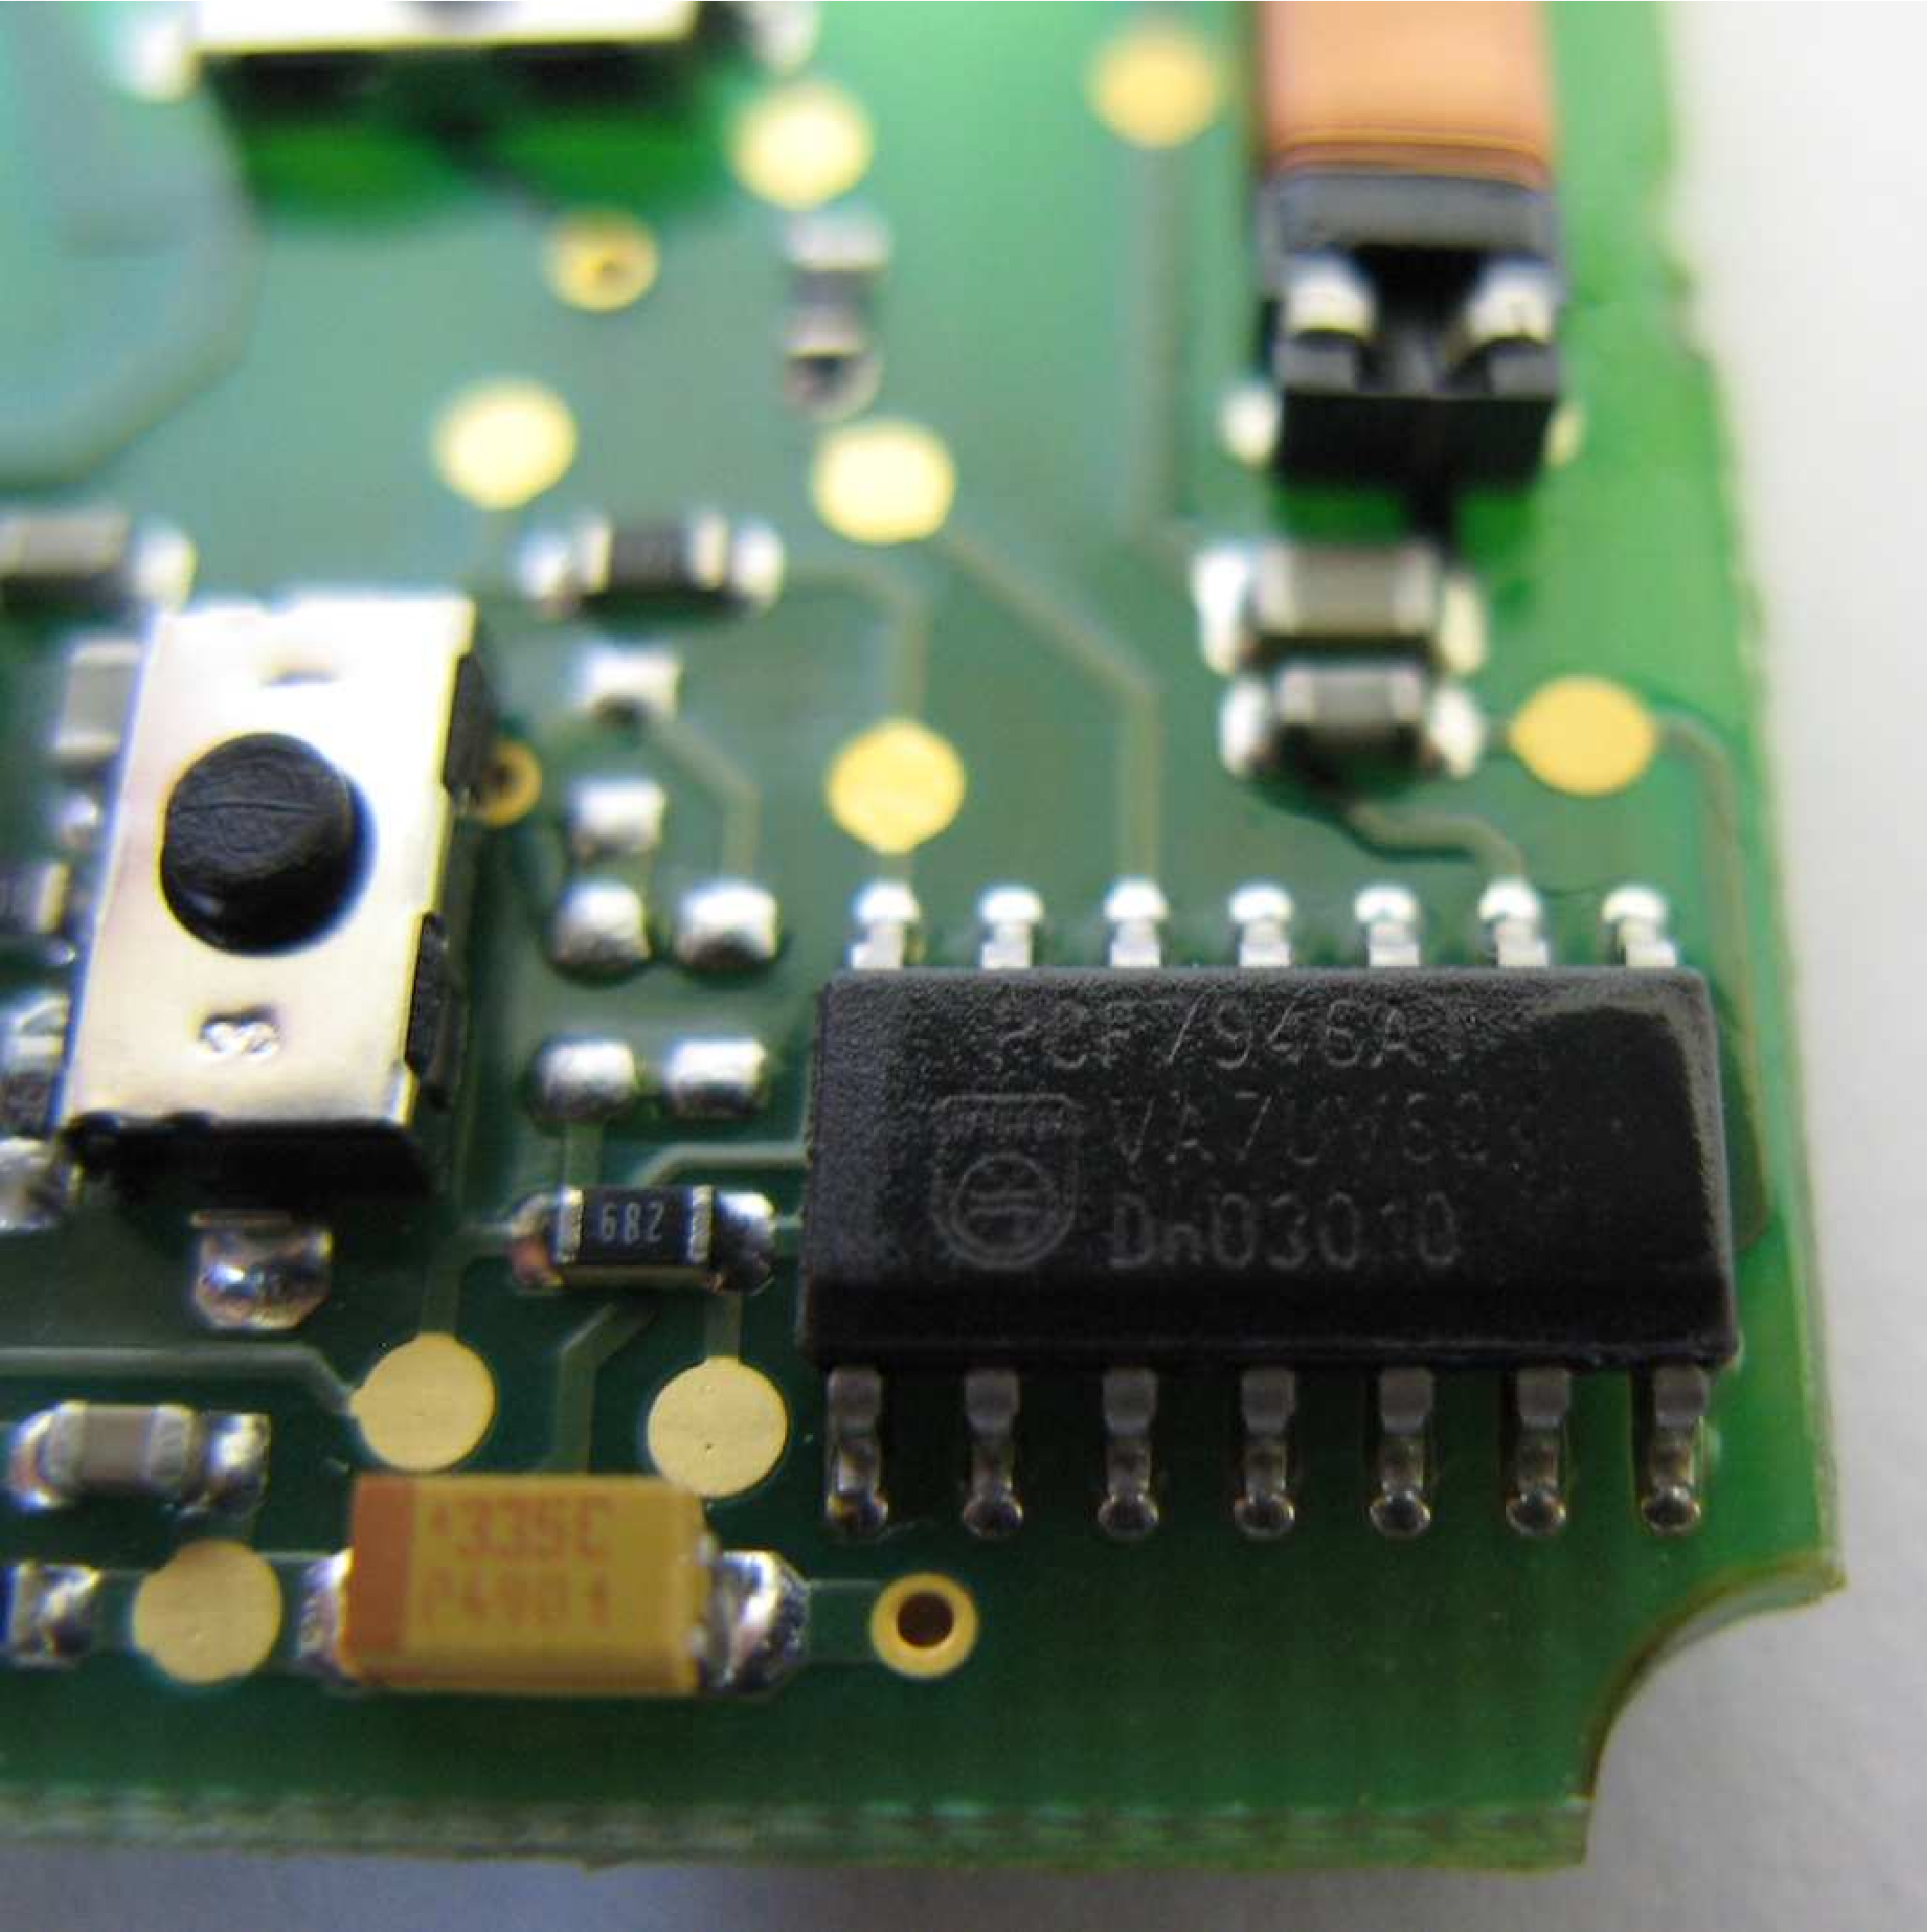
\includegraphics[width=2.35in]{images/NissanSchluessel2}
  }
  \caption{This figure shows a Nissan car key and the transponder used. Clearly visible is the antenna for 125\,kHz (very thin copper wire on ferrite core).}
  \label{fig:keys}
 \end{figure} %
\begin{figure}[p]
 \ContinuedFloat
  \centering
  \hfill %
  \subfloat[Carbon type transponder.]{
      %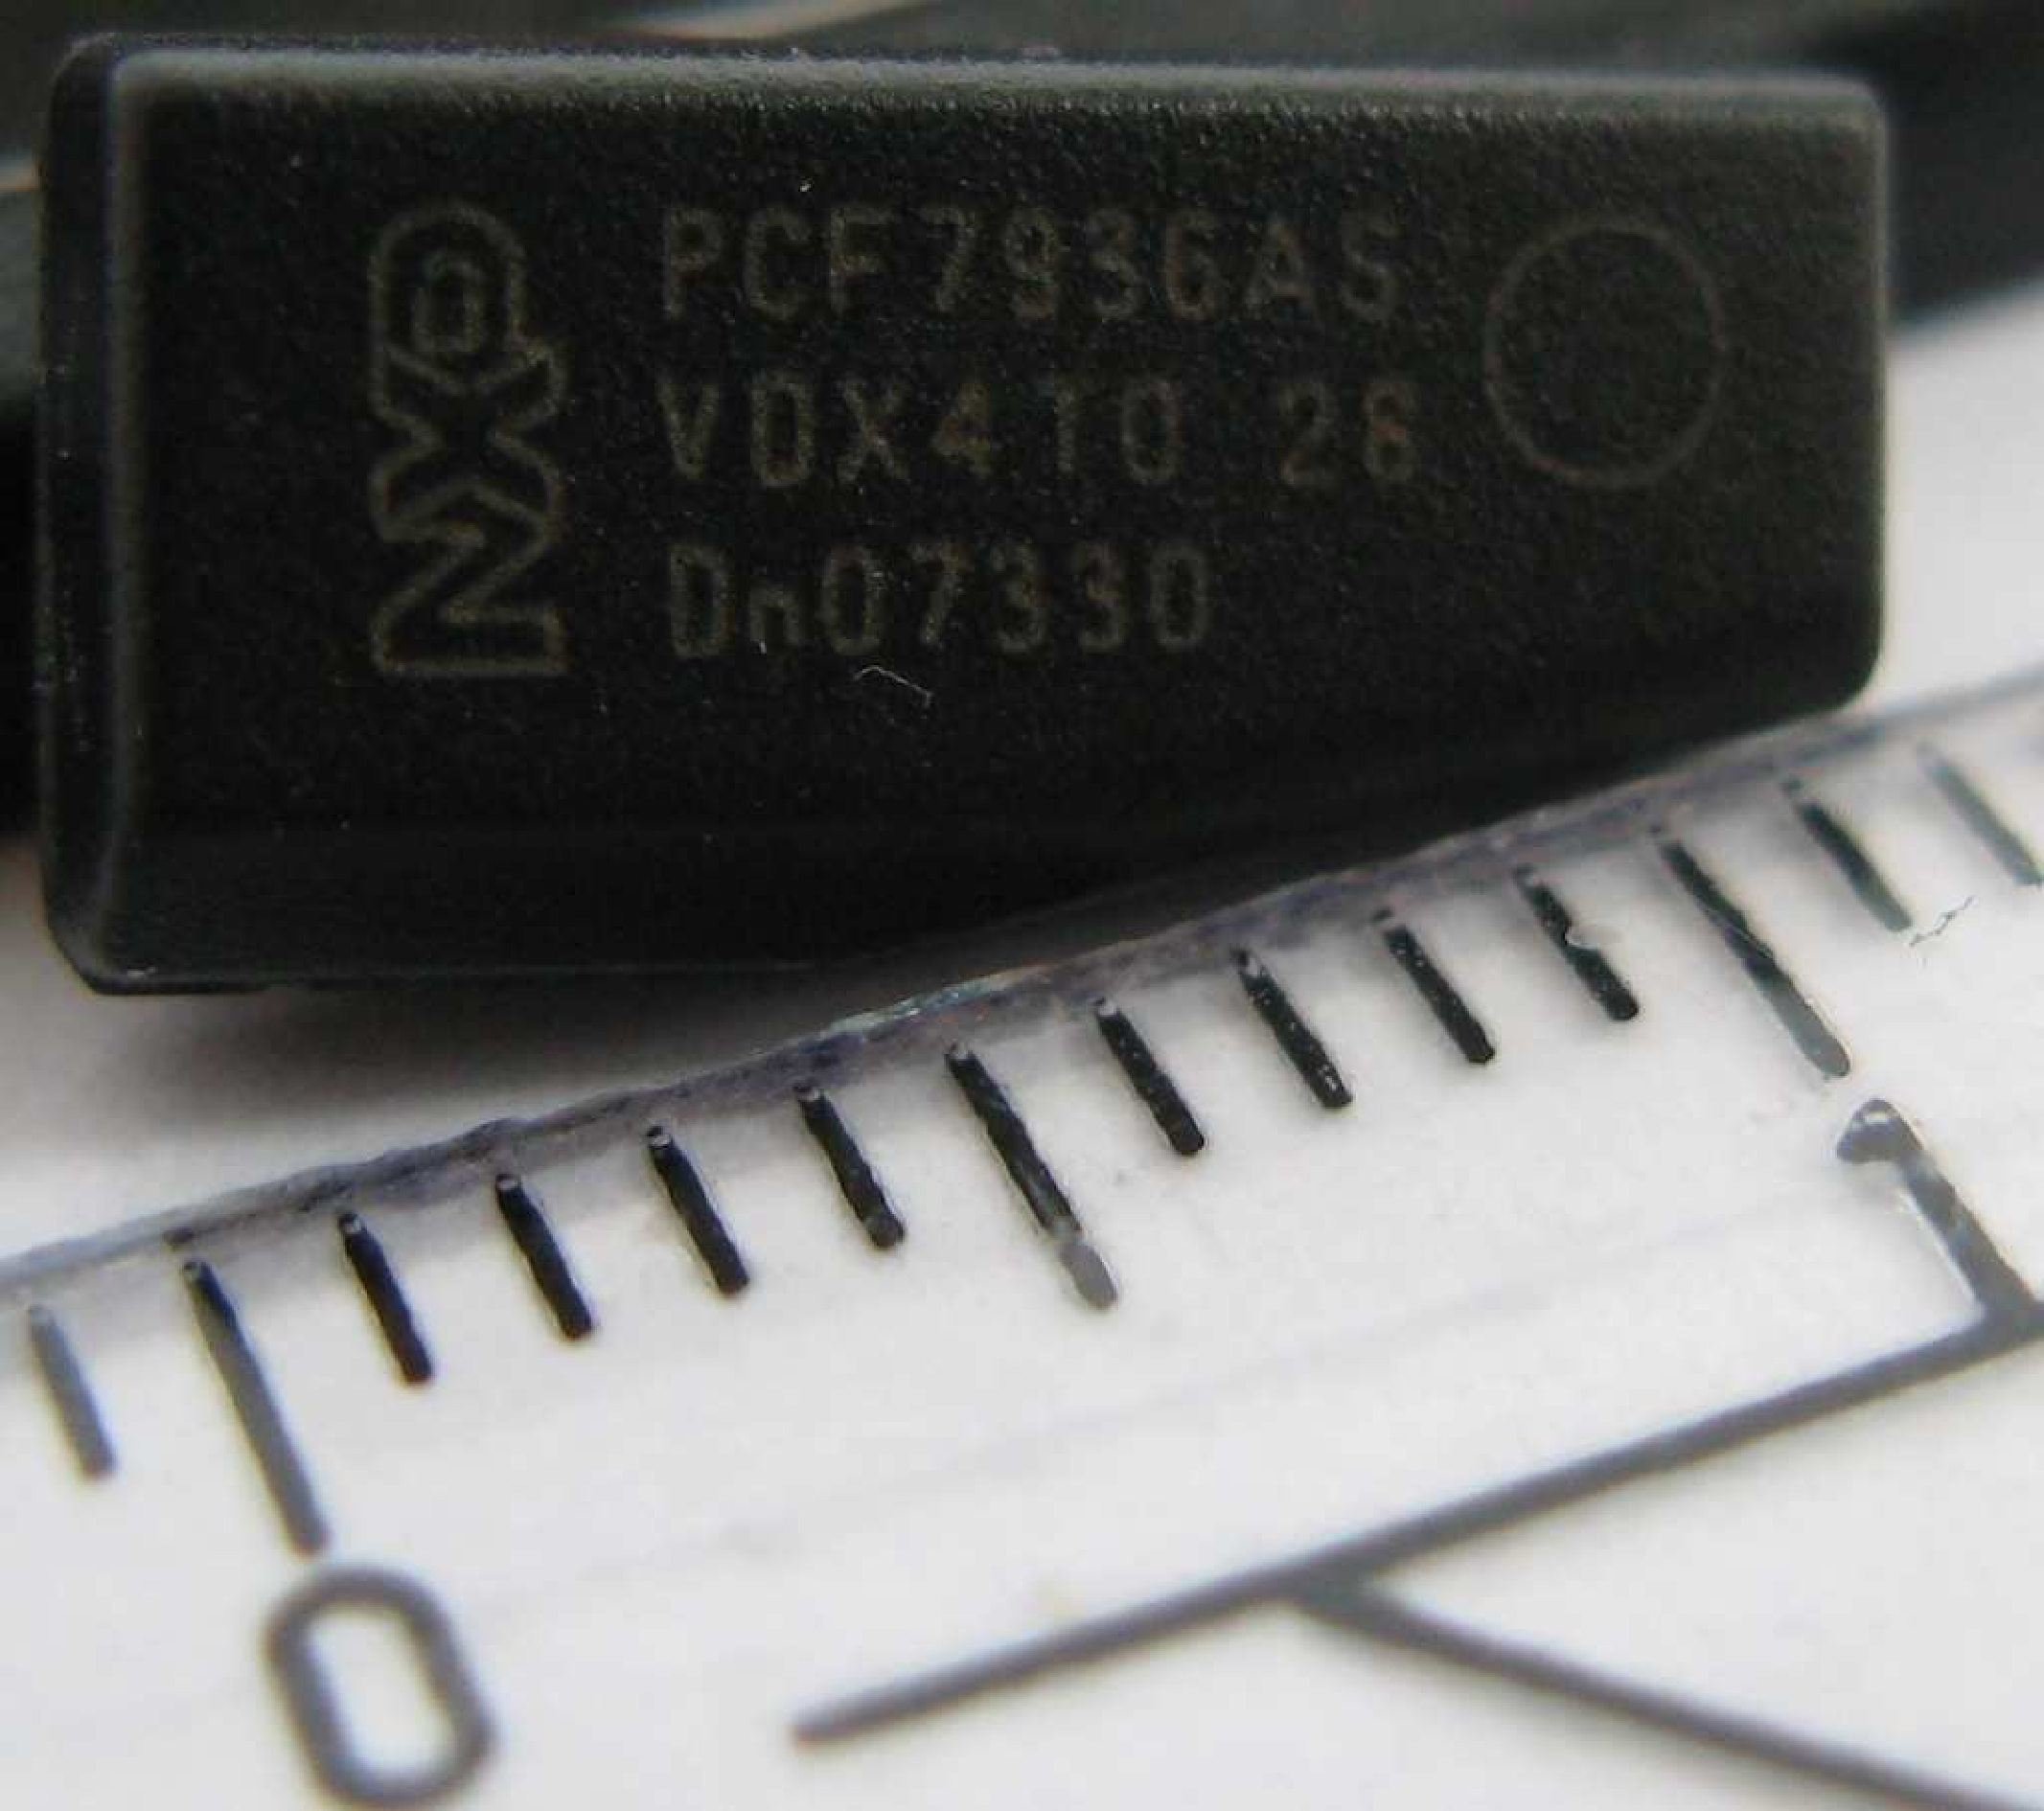
\includegraphics[width=2.35in]{images/PCF7936a}
  }
  \hfill %
  \subfloat[Disc type transponder.]{
      %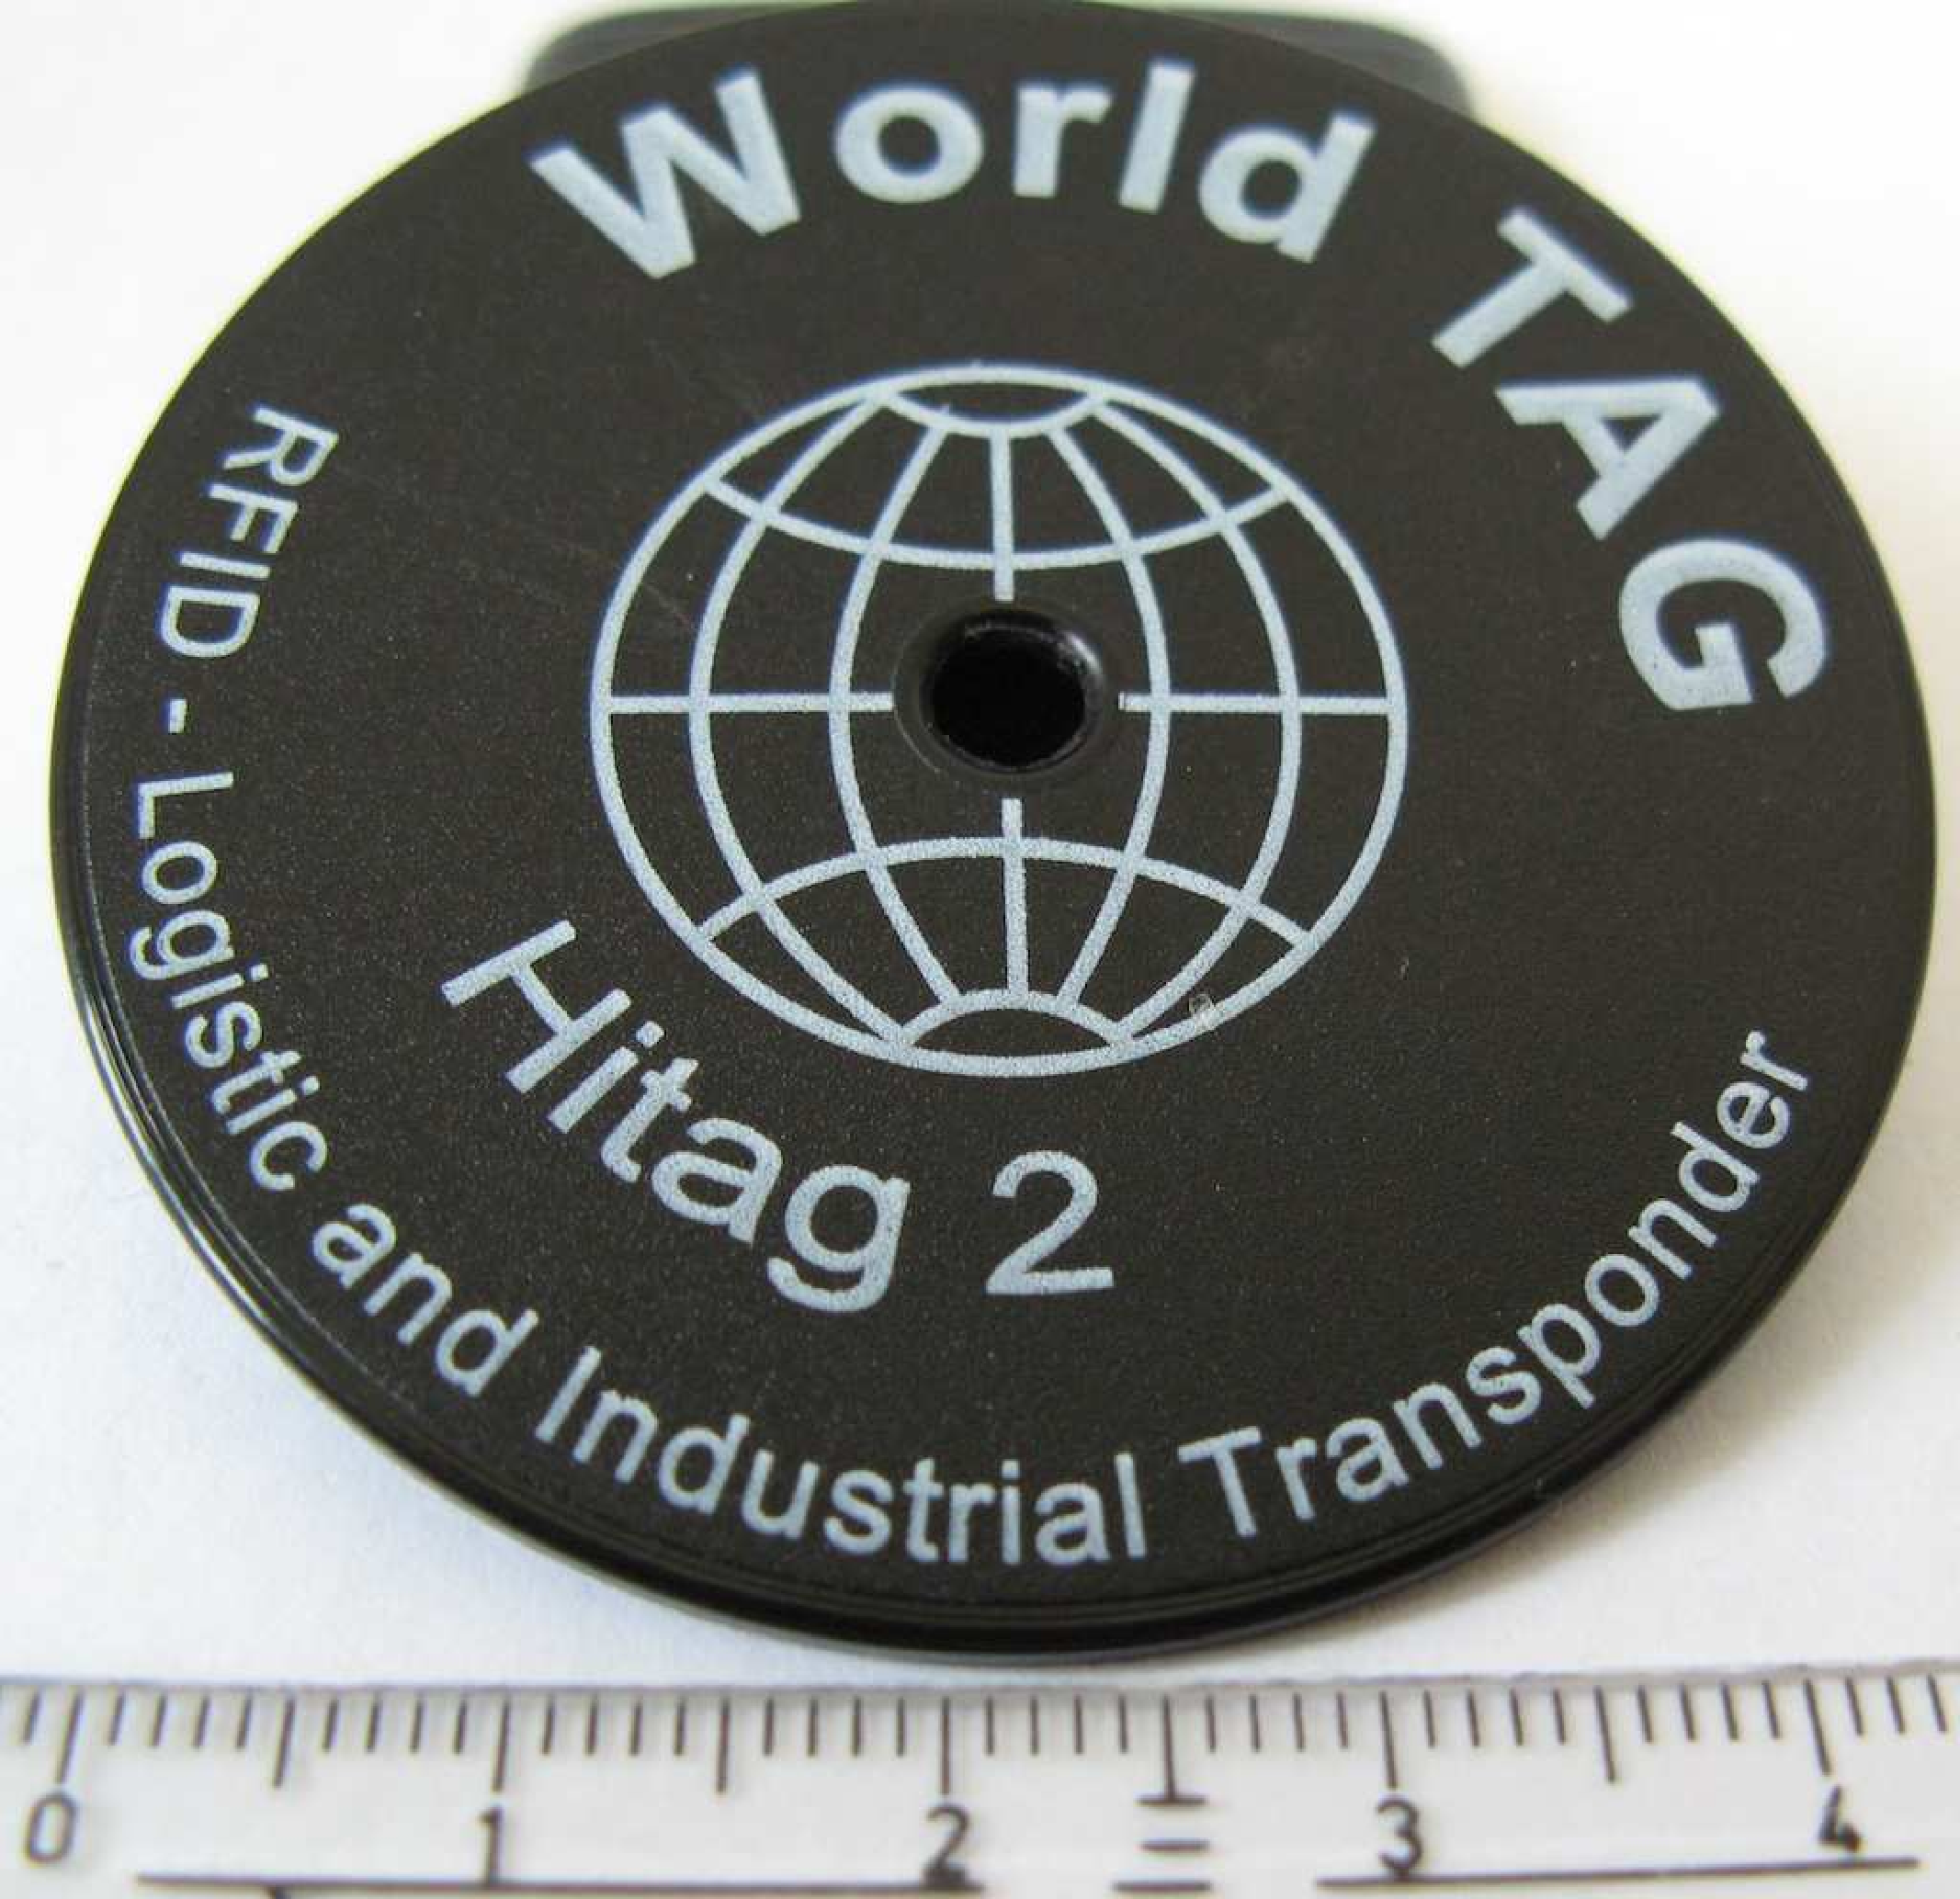
\includegraphics[width=2.35in]{images/WorldTag}
  }
  \caption{Two out of many possible shapes of PCF7936 transponders. Unit of measurement is centimeter.}
  %\label{fig:keys}
\end{figure} %

\clearpage

\subsubsection{Tables}

There are many possibilities on how to create and include tables. From a typographic point of view, \textit{one should avoid any vertical lines}, cf. Table~\ref{tab1}.


\begin{table}[htbp]
	\centering
	\begin{minipage}{\textwidth} % only needed for footnotes, otherwise footnotes will not appear
	\renewcommand{\footnoterule}{}
 	\renewcommand{\thefootnote}{\alph{footnote}}
	\centering
	\caption[This is the short caption for the \textit{List of Tables}.]{Captions for tables are \emph{always above} the table and give a short but informative description of the table. Always use full sentences here and end them with a full stop.}
	\label{tab1}
	\begin{tabular}{@{}lccc@{}} \toprule
	& & \multicolumn{2}{c}{Component}\\
	\cmidrule{3-4}
	Amount\footnote{This is a footnote inside a table, you need a minipage for this to work.} & Price & Description & Role \\
	\midrule
	23 & 1.234 \$ & good stuff & important\\
	\midrule
	multirow example & \multirow{2}{*}{x} & \multirow{2}{*}{y} & \multirow{2}{*}{XXX} \\
	the other row & & &\\
	\midrule
	42 & 43.123,13\footnote{This is another footnote inside a table.} & good stuff & important\\
	\bottomrule
	\end{tabular}
	\end{minipage}
\end{table}


\subsubsection{Definitions}

This is a definition. You can of course make a reference to it~\ref{def1}.

\begin{definition}[A name]\label{def1}
 A really good definition. Lorem ipsum dolor sit amet, consetetur sadipscing elitr, sed diam nonumy eirmod tempor invidunt ut labore et dolore magna aliquyam erat, sed diam voluptua. At vero eos et accusam et justo duo dolores et ea rebum. Stet clita kasd gubergren, no sea takimata sanctus est Lorem ipsum dolor sit amet.
\end{definition}


\subsection{Listings, Algorithms}

\subsubsection{Listings}
For source code listings, three options are available:
\begin{itemize}
\item the \texttt{verbatim} environment,
\item the \texttt{listings} package,
\item and the \texttt{lgrind} package.
\end{itemize}

The verbatim environment is the most simple environment and not suited for large code listings (due to different limitations). Only use it for single

\begin{verbatim}
$ important shell commands
\end{verbatim}

Otherwise, either use the \texttt{listings} or \texttt{lgrind} packages. The listings package is easier to use, therefore we present it here. \emph{Important} advice: Only explain important functions and/or structures of your program in your thesis..Especially point out the big picture of your program, for instance, how different modules interact and which important input limitations to respect. Please note: Using special language characters (\^{e},\/ \"{u},\/ \"{a}, \dots) in your source code is strongly discouraged, as they may cause problems using the \texttt{listings} package.

\begin{lstlisting}[language={C}, caption={A sample listing of a C function. Description of the function is here. Please note that different languages are available.}, numbers=left]
/*!
 * This is a Doxygen comment for a function.
 * \param first operand
 * \param second operand
 * \returns a+b
 */
int  sum(int a, int b)
{
	return (a + b);
}
\end{lstlisting}

\begin{lstlisting}[language={VHDL}, caption={A sample listing of a VHDL entity. Description of the entity is here. Please note that different languages are available.}, numbers=left]
entity InterLeavedMul is
	generic(wide  : natural :=8); -- highest bit
  port(clk  : in std_logic;
       rst  : in std_logic;
       x    : in std_logic_vector(wide-1 downto 0);
       y    : in std_logic_vector(wide-1 downto 0);
       N    : in std_logic_vector(wide-1 downto 0);
			 start: in std_logic;
       done : out std_logic;
       xyN  : out std_logic_vector(wide-1 downto 0));
end  InterLeavedMul;
\end{lstlisting}

You should thoroughly document your code using comments and (best case) by using a documentation system like Doxygen. Please ask your supervisor for additional rules (e.\,g. which repository system to use, etc.). Regularly commit your changes and backup your data!

\subsubsection{Algorithms}

For many theses, typesetting algorithms is necessary. There are at least four packages available that allow easy typesetting of algorithms.

\begin{itemize}
\item \texttt{program} offering the environment \texttt{program}.
\item \texttt{algorithm} offering the environment \texttt{algorithm}.
\item \texttt{algorithmic} offering the environment \texttt{algorithmic}.
	\begin{itemize}
	\item This package sometimes has compatibility problems with \texttt{hyperref}.
	\end{itemize}
\item \texttt{algorithm2e} either offering the environment \texttt{algorithm} or \texttt{algorithm2e}.
\end{itemize}

Students are advised to use only \emph{one} of these packages and not mix them. The author of this template suggests to use the package \texttt{algorithm2e} with the option \texttt{algo2e}. This prevents conflicts with other packages, just in case it is ever required to mix \texttt{algorithm} or \texttt{algorithmic} with \texttt{algorithm2e}.

\begin{algorithm2e} 
\KwData{unsorted array $A[1 \ldots n]$}
\KwResult{array $A[1 \ldots n]$ with $A[1] \leq A[2] \leq \ldots \leq A[n]$}
\caption{\textsc{Insertion-Sort}}

\Begin{ 
\For{$j \leftarrow 2$ \KwTo $\mathrm{length}[A]$}{
$key \leftarrow A[j]$\;
\tcc{Insert $A[j]$ into the sorted sequence $A[1 \ldots j -1]$}
$i \leftarrow j - 1$\;
\While{$i > 0$ \KwSty{and} $A[i] > key$}{\;
$A[i+1] \leftarrow A[i]$\;
$i \leftarrow i-1$
}
$A[i+1] \leftarrow key$
} 
}
\end{algorithm2e}

\clearpage

\subsection{Protocols}

\subsubsection{2-Party Protocol Sessions}
\begin{figure}[!htb]
\fbox{\begin{minipage}{\textwidth}%
\begin{protocol}{2}
\participants{\textbf{Reader}}{\textbf{Transponder}} \\ 
					& \sends{\texttt{Start\_Auth} \texttt{[11000]}}		    				 &	\\
                                      	&  \receives{\texttt{Header [11111], Serial Number [31..0]}}			 & \\
\texttt{compute Auth$_B$}&  \sends{\texttt{IV [31..0], Auth$_B$ [31..0]}}						 & \texttt{compute Auth$_T$} \\
\texttt{generate IV}		& 														 & \texttt{Auth$_B \stackrel{?}{=}$ Auth$_T$}\\
	                                      &  \receives{\texttt{Header [11111], Page 3 [31..0]$_{k}$}}			 & \\
\end{protocol}
\end{minipage}}%
\caption{Mutual authentication of the HITAG~2 protocol in crypto mode.}
\label{fig:authcrypto}
\end{figure}

\subsubsection{Protocol Headers}

\begin{figure}[!htb]
\begin{center}
\begin{bytefield}[bitwidth=1.8em]{16}\\
\bitheader{0-15} \\
\wordbox{1}{ID} \\
\bitbox{1}{{QR}} & \bitbox{4}{Opcode} & \bitbox{1}{AA} & \bitbox{1}{TC} & \bitbox{1}{RD} & \bitbox{1}{RA}
\bitbox{3}{Z} & \bitbox{4}{RCODE} \\
\wordbox{1}{QDCOUNT} \\
\wordbox{1}{ANCOUNT} \\
\wordbox{1}{NSCOUNT} \\
\wordbox{1}{ARCOUNT} \\
\end{bytefield}
\caption{DNS Request}
\end{center}
\label{fig:dnsheader}
\end{figure}

